\documentclass[11pt,twoside]{article}
\usepackage{geometry}
\usepackage{enumerate}
\usepackage{latexsym,booktabs}
\usepackage{amsmath,amssymb}
\usepackage{graphicx}
\usepackage[colorlinks, linkcolor = blue]{hyperref}
\usepackage[singlespacing]{setspace}
\usepackage{calc}
\usepackage{multirow}


\geometry{a4paper,left=2cm,right=2.0cm, top=2cm, bottom=2.0cm}

\newtheorem{Definition}{Definition}
\newtheorem{Theorem}{Theorem}
\newtheorem{Lemma}{Lemma}
\newtheorem{Corollary}{Corollary}
\newtheorem{Proposition}{Proposition}
\newtheorem{Algorithm}{Algorithm}
\numberwithin{Theorem}{section}
\numberwithin{Definition}{section}
\numberwithin{Lemma}{section}
\numberwithin{Algorithm}{section}
\numberwithin{equation}{section}

\newcommand{\dottedline}[1]{\makebox[#1]{.\dotfill}}

\begin{document}
	
\pagestyle{empty}

 %=============================================================================
 %Title page
 %=============================================================================
\begin{titlepage}
\vspace*{.5em}
\centering
\textbf{\Large{The School of Mathematics}} \\
\vspace*{1em}
\begin{figure}[!h]
\centering

\includegraphics[width=180pt]{CentredLogoCMYK.jpg}
\end{figure}
\vspace{2em}
\textbf{\Huge{Analysis on Risk Factors for Leptospirosis Based on Generalized Linear Mixed Models}}\\[2em]
\textbf{\LARGE{by}}\\
\vspace{2em}
\textbf{\LARGE{Yile Shi}}\\
\vspace{6.5em}
\Large{Dissertation Presented for the Degree of\\
MSc in Statistics with Data Science}\\
\vspace{6.5em}
\Large{August 2021}\\
\vspace{3em}
\Large{Supervised by\\Dr. Gail Robertson and Dr. Amy Wilson}
\vfill
\end{titlepage}

\clearpage

% =============================================================================
% Executive summary, acknowledgments, and own work declaration
% =============================================================================
\begin{center}
\Large{Executive Summary}
\end{center}

\textbf{Background:} Leptospirosis, a widely distributed zoonotic disease, has become a major public health concern due to its significant effect on human and animal morbidity and mortality \cite{haake2015leptospirosis}. Although various researches have been conducted to study this zoonotic infection in different domains, work on identifying individuals at risk, especially in low-income rural areas in developing countries, is still deficient.

\

\textbf{Research question:} This research aims to shed light on the potential risk factors that affect individual's leptospirosis infection in a rural area of Kenya, and further generate knowledge to help inform health intervention programmes for leptospirosis infections reduction. We consider 8 explanatory variables: gender, age, land use, occupation, distance to local hospital, altitude, family size, and occupation of household head, as well as 3 environmental variables with nested structures.

\

\textbf{Data:} We use a subset with 595 subjects of the sampled data collected by the International Livestock Research Institute from members of households in villages in Tana River County, Kenya, including the leptospirosis test results using ELIZA (enzyme-linked immunosorbent assay). 


\

\textbf{Methods:} We construct binomial generalized linear mixed models including the random effect of environmental variables, where the response of interest is individual's ELIZA teste result. The random intercept model with village effect is selected due to its best performance by AIC (Akaike Information Criterion). Moreover, we conduct model diagnosis and evaluation, including residual plots and ROC (Receiver Operating Characteristic) curves (Figure \ref{fig:ROC}). 

\

\textbf{Results:} We obtain the random intercept among villages is normally distributed with mean 0 and standard deviation 0.5053. Considering the village effect, gender, land use (at 0.1 significance level) and occupation of household head tend to have significant effects on individual's leptospirosis infection. Specifically, male individuals (OR 0.6427; 95\% CI 0.4194 to 0.9764) have less risk for leptospirosis seropositivity than female individuals; people working on pastoral land (OR 0.3582; 95\% CI 0.1151 to 1.1372) or riverine land (OR 0.5738; 95\% CI 0.1657 to 1.8141) are less likely to be infected, comparing with irrigation land group; individuals with household heads working as pastoralists (OR 6.4987; 95\% CI 2.2190 to 19.3265) take more risk for leptospirosis seropositivity than farmers group.

\begin{figure}[!h]
	\centering
	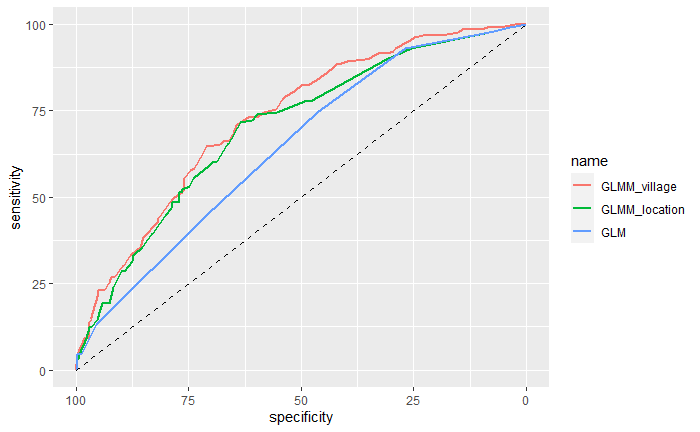
\includegraphics[width = 0.75\textwidth]{Images/ROC.png}
	\caption{ROC curves of different models}
	\label{fig:ROC}
\end{figure}

\clearpage

\begin{center}
\Large{Acknowledgments}
\end{center}

I am sincerely grateful to the supervisors of this project, Dr. Gail Robertson and Dr. Amy Wilson, as well as PhD supporter Miss. Rebecca Akeresola, for their advice and guidance. I would also like to thank the International Livestock Research Institute for providing the data and background information used in the research. 

\clearpage


\begin{center}
\Large{University of Edinburgh – Own Work Declaration}
\end{center}

This sheet must be filled in, signed and dated - your work will not be marked unless this is done.
\vspace{1cm}

Name: Yile Shi

Matriculation Number: s2168022

Title of work: Analysis on Leptospirosis Risk Factors Based on Generalized Linear Mixed Model

\vspace{1cm}

We confirm that all this work is my own except where indicated, and that We have:
\begin{itemize}
\item	Clearly referenced/listed all sources as appropriate	 				
\item	Referenced and put in inverted commas all quoted text (from books, web, etc)	
\item	Given the sources of all pictures, data etc. that are not my own				
\item	Not made any use of the report(s) or essay(s) of any other student(s) either past 	
or present	
\item	Not sought or used the help of any external professional academic agencies for the work
\item	Acknowledged in appropriate places any help that We have received from others	(e.g. fellow students, technicians, statisticians, external sources)
\item	Complied with any other plagiarism criteria specified in the Course handbook
\end{itemize}

We understand that any false claim for this work will be penalised in accordance with
the University regulations	(\url{https://teaching.maths.ed.ac.uk/main/msc-students/msc-programmes/statistics/data-science/assessment/academic-misconduct}).								

\vspace{1cm}

Signature:

\begin{figure}[!h]
	
\includegraphics[width = 0.5\textwidth]{Images/Signature.png}
\end{figure}

\vspace{5mm}

Date: 2022/8/10

\clearpage


% =============================================================================
% Table of contents, tables, and pictures (if applicable)
% =============================================================================
\pagestyle{plain}
\setcounter{page}{1}
\pagenumbering{Roman}

\tableofcontents

\pagenumbering{arabic}
\setcounter{page}{1}

\nocite{*}
\bibliographystyle{unsrt}
\clearpage

\section{Introduction}
\label{sec:intro}

Leptospirosis, a zoonosis found worldwide, remains a major public health issue in many developing countries, which is expected to become more important due to a rapid urbanization, global warming, and extreme climatic events such as floods \cite{picardeau2013diagnosis}. Due to the difficulty of accurate data collection, identification of risk factors for individual's leptospirosis infection in rural areas of developing countries becomes an active research topic. This report aims to contribute to this topic by exploring potential risk factors behind leptospirosis diagnosis. We expect that a better understanding of the influence of factors on leptospirosis infection can help to inform the development of lifestyle interventions for leptospirosis risk reduction. 

We apply exploratory data analysis (EDA) on sampled data collected by the International Livestock Research Institute from members of households in villages in Tana River County, Kenya, and extract a subset of 595 individuals with 11 columns as well as the leptospirosis test results using ELIZA (enzyme-linked immunosorbent assay). We build generalized linear mixed models including the random effect of environmental variables, and select the best performed one. Our goal is to find, among the following potential risk factors, the most likely to be relevant to leptospirosis seropositivity, with an environment effect into consideration: gender; age; land use; occupation; distance to local hospital; altitude; family size; and occupation of household head.

\section{Exploratory Data Analysis}  
\label{sec: EDA}

\subsection{Missing Data}

We detect a serious problem of missing values in the dataset after dropping duplicated data. Table \ref{tab:missing} displays the number and proportion of missing values, arranged in descending order. 

\begin{table}[!h]
	\centering
	\begin{tabular}{|c|c|c|}
		\hline
		variable & count & proportion \\
		\hline
		\texttt{occupation} & 343 & 0.3649 \\ 
		\texttt{disthosp} &259 & 0.2755 \\
		\texttt{livestk\_home}  &  236 & 0.2511 \\
        \texttt{location}  &  236 & 0.2511 \\
		\texttt{landuse} & 4 & 0.0043 \\
		\texttt{gender} & 1 & 0.0011 \\
		\texttt{age} & 1 & 0.0011 \\
		\hline
	\end{tabular}
	\caption{Number and proportion of missing values in variables}
	\label{tab:missing}
\end{table}

\texttt{landuse}, \texttt{gender} and \texttt{age} contain missing values less than 1\% and we drop the corresponding observations without much loss of information of the original dataset. 

According to data description, \texttt{livestk\_home} is a binary variable indicating whether or not livestock is kept in the household of sampled person. Although contact with animals increases risk of leptospirosis \cite{cook2017risk}, from figure \ref{fig:livestk}, we observe a significant imbalance, which probably leads to insignificant results. Thus, we exclude this column from further modelling.

\begin{figure}[!h]
	\centering
	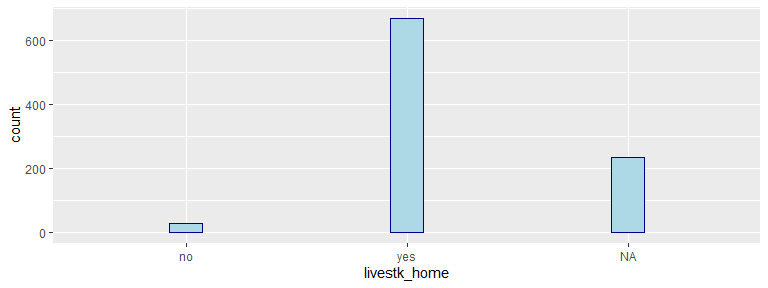
\includegraphics[width = 0.75\textwidth]{Images/livestk.png}
	\caption{Distribution of \texttt{livestk\_home}}
	\label{fig:livestk}
\end{figure}

\texttt{disthosp} is the Euclidean distance from the sampled person's household to local hospital. Here, we assume that people from the same village go to the same hospital. Then, we impute the missing values with the mean distance to the local hospital of each village. However, we observe that data in \texttt{disthosp} in village 12, 13 and 23 are completely missing and fail to impute. Instead, we drop corresponding rows in these villages. 

\texttt{location} is the anonymised location of area where sampling was done. Again, we consider using \texttt{village} to determine the corresponding location in the same row. However, we still meet the problem that data in \texttt{locations} in some villages are completely missing. Besides, we observe that subjects from the same village could belong to different locations. possibly because the village is on the boundary of two locations or it is just a mistake in data input. As a result, we drop all missing values in this column instead of imputation.

Individual's occupation could have great influence on leptospirosis infection \cite{cook2017risk}, associated with various aspects. Figure \ref{fig:occ1} shows the conditional distributions of \texttt{occupation} in juvenile (< 18 yeas old) and adult ($\geq$ 18 years old) groups. 

\begin{figure}[!h]
	\centering
	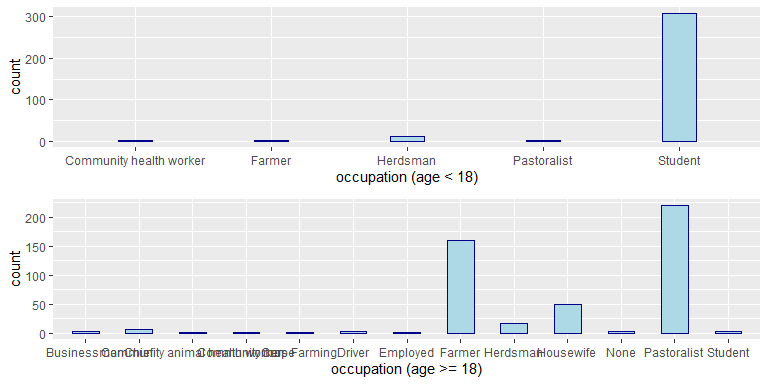
\includegraphics[width = 0.75\textwidth]{Images/occupation_age.png}
	\caption{Distribution of \texttt{occupation}, conditioning on \texttt{age}}
	\label{fig:occ1}
\end{figure}

It is shown that juveniles are most likely to be students, hence we impute the missing occupation for juvenile individuals with "Student". However, the case for adults is complicated. A p-value $<2.2e-16$ from the $\chi^2$ test shows strong evidence that individual's occupation is correlated with the type of land use. We also observed this relationship in Figure \ref{fig:occ3}. Specifically, most sampled adults working on irrigation or riverine land are farmers, while individuals pastoral land are most likely to be pastoralists. Besides, \texttt{gender} and \texttt{constituency} are also observed to be correlated with \texttt{occupation}. 

It is hard to determine an appropriate imputation method for adult group. Instead, we drop adult subjects missing in \texttt{occupation}.

\begin{figure}[!h]
	\centering
	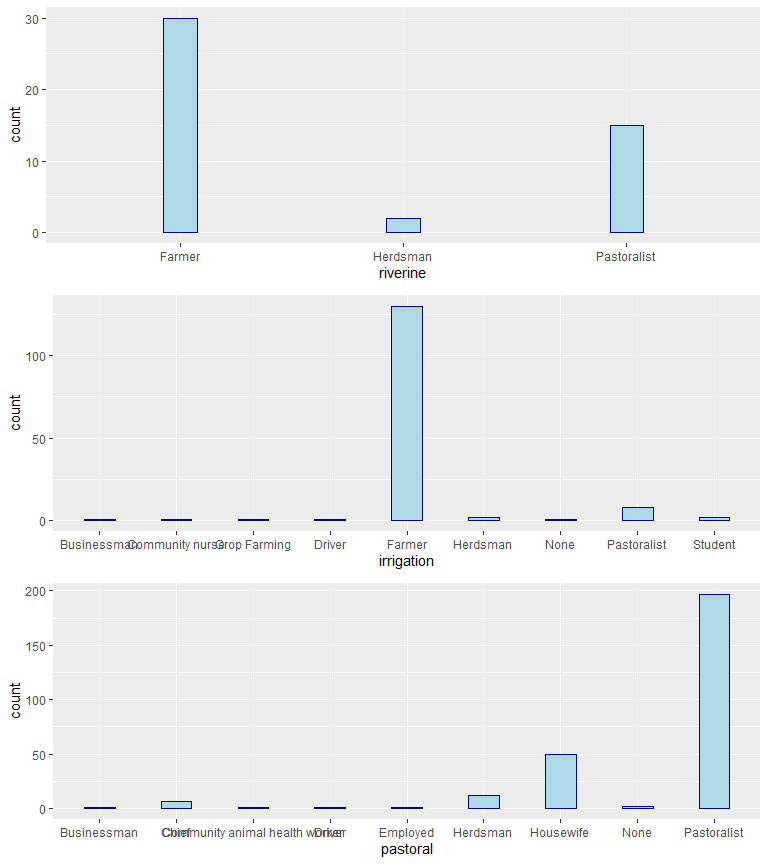
\includegraphics[width = 0.75\textwidth]{Images/occupation_landuse.png}
	\caption{Ddistributions of \texttt{occupation} in adult group, conditioning on \texttt{landuse}}
	\label{fig:occ3}		
\end{figure} 

\subsection{Feature Selection}

We now determine the columns used for modelling. \texttt{result}, which represents whether the sample individual is leptospirosis seropositive or not based on ELISA (enzyme-linked immunosorbent assay), is considered as the response variable. 

As for potential risk factors, identifier columns including \texttt{sampleid} and \texttt{parent} are excluded from our model, as well as \texttt{relationshiphh} and \texttt{genhhid}. Besides, as mentioned before, we do not take \texttt{livestk\_home} into consideration. We select features from the rest columns based on plots and the work of Goarant et al (2016) \cite{goarant2016leptospirosis}. 

\subsubsection{Nominal Variables}

We start with nominal variables \texttt{gender}, \texttt{occupation}, \texttt{landuse}, \texttt{hhoccup} and \texttt{hhgender}. First, we count the number of observations in each category of \texttt{occupation} and \texttt{hhoccup}, the occupation of household head, grouped by two columns respectively.

\begin{table}[!h]
	\centering
	\begin{tabular}{|l|l|l|l|}
		\hline
		\multicolumn{2}{|c|}{\texttt{occupation}} & \multicolumn{2}{|c|}{\texttt{hhoccup}} \\
		\hline
		category & 	count & category & count \\
		\hline
		Student & 239 & Pastoralist & 345 \\				
		Pastoralist & 159 & Farmer & 247 \\
		Farmer & 156 & Chief & 15 \\
		Housewife & 36	& Businessman & 5 \\			
		Herdsman & 20 & Civil Servant & 4 \\	
		Chief & 6 & Herdsman & 3 \\	
		Businessman & 2 & Crop Farming & 2 \\
		Driver & 2 & None & 2 \\
		Community animal health worker & 1 & Casual Labourer & 1 \\			
		Community nurse & 1	& Driver & 1 \\	
		Crop Farming & 1 & & \\			
		Employed & 1 & & \\
		None & 1 & & \\
		\hline
	\end{tabular}	
	\caption{Number of observations in each category in \texttt{occupation} and \texttt{hhoccup}}
	\label{tab:occ}
\end{table}

 As shown in Table \ref{tab:occ}, most categories contain observations less than 20. Small and insufficient group size would lead to unstable and biased results. On the other hand, numerous occupation groups could result in larger degrees of freedom, which increases model complexity. As a remedy, we merge occupation groups with similar meanings and risks of exposure, such as "Crop Farming" and "Farmer", "Herdsman" and "Pastoralist". However, most smaller occupation groups have very different risk profiles, e.g. drivers are unlikely to have the same contact with animal risk as farmers. In this case, we disregard such categories and discard corresponding observations.

We plot stacked bar charts for nominal variables and report the prevalence in each category. From Figure \ref{fig:factor} and Table \ref{tab:factor}, \texttt{gender},  \texttt{occupation}, \texttt{landuse} and \texttt{hhoccup} have significantly different prevalence among categories, hence we select them as feature candidates for modelling. Although \texttt{hhgender} also tends to have significant effect, we exclude this column due to its imbalance where over 80\% observations are males.

\begin{figure}[!h]
	\centering
	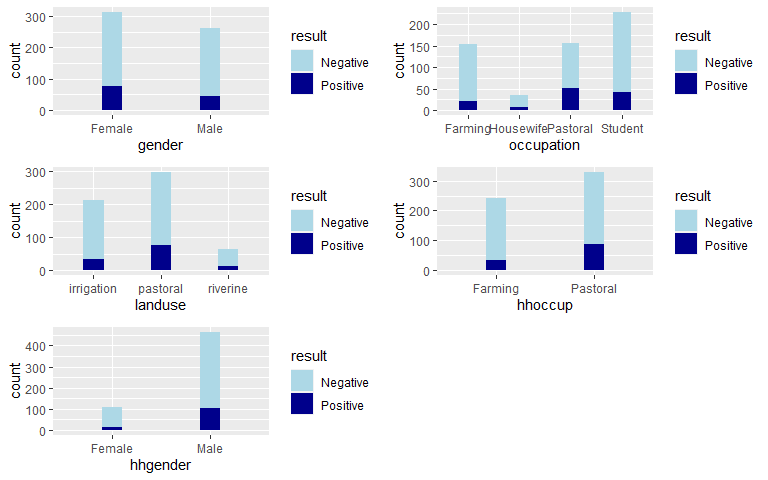
\includegraphics[width = \textwidth]{Images/factors.png}
	\caption{Stacked bar plot of \texttt{result} in factor variables}
	\label{fig:factor}
\end{figure}

\begin{table}[!h]
	\centering
	\begin{tabular}{|c|c|c|}
		\hline
		factor & category & prevalence \\
		\hline
		\multirow{2}{*}{\texttt{gender}} & Female & 0.2508 \\
		 & Male & 0.1821 \\
		\hline
		\multirow{4}{*}{\texttt{occupation}} & Farmer & 0.1465 \\
		 & Student & 0.1834 \\			
		 & Pastoralist & 0.3257 \\			
		 & Housewife & 0.2353 \\
		\hline
		\multirow{3}{*}{\texttt{landuse}} & irrigation & 0.1636 \\
		 & pastoral & 0.2597 \\
		 & riverine & 0.2090 \\
		\hline
		\multirow{2}{*}{\texttt{hhoccup}} & Farmer & 0.1325 \\
		 & Pastoralist & 0.2803 \\
		\hline
		\multirow{2}{*}{\texttt{hhgender}} & Female & 0.1481 \\
		 & Male & 0.2341 \\
		\hline
	\end{tabular}
	\caption{Prevalence in each category of factor variables}
	\label{tab:factor}
\end{table}

\subsubsection{Numerical Variables}

We make box plots for numerical variables including \texttt{age}, \texttt{altitude}, \texttt{nmales}, \texttt{nfemales}, \texttt{famsize} and \texttt{disthosp}, grouped by \texttt{result}. 

\begin{figure}[!h]
	\centering
	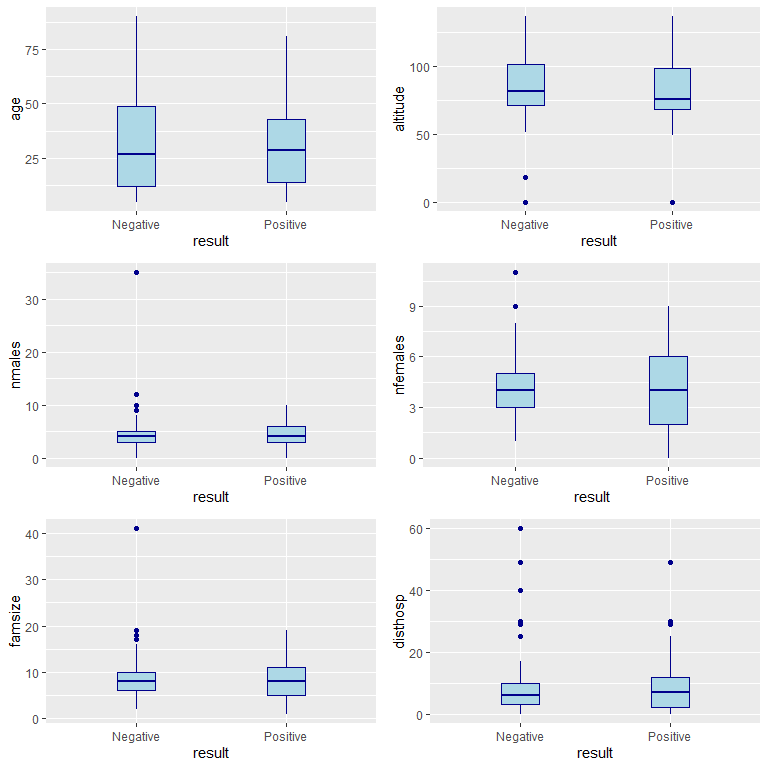
\includegraphics[width = 0.8\textwidth]{Images/numerical.png}
	\caption{Box plots of numerical variables, grouped by \texttt{result}}
	\label{fig:numerical}
\end{figure}

Comparing with nominal variables, numerical variables do not show such significantl difference between "Negative" and "Positive" groups in Figure \ref{fig:numerical}. Based on \cite{goarant2016leptospirosis}, we select \texttt{age}, \texttt{altitude}, \texttt{famsize}, the number of people in the sampled household and \texttt{disthosp} as feature candidates for modelling. 

\subsubsection{Environmental Variables}

Environmental variables including \texttt{village}, \texttt{location} and \texttt{constituency} indicate the geographical information of sampled people, with an order $\texttt{village} < \texttt{location} < \texttt{constituency}$.  Again, we plot the stacked bar charts of the response variable and compute the prevalence, grouped by the levels in \texttt{village}, \texttt{location} and \texttt{constituency} respectively. 

\begin{figure}[!h]
	\centering
	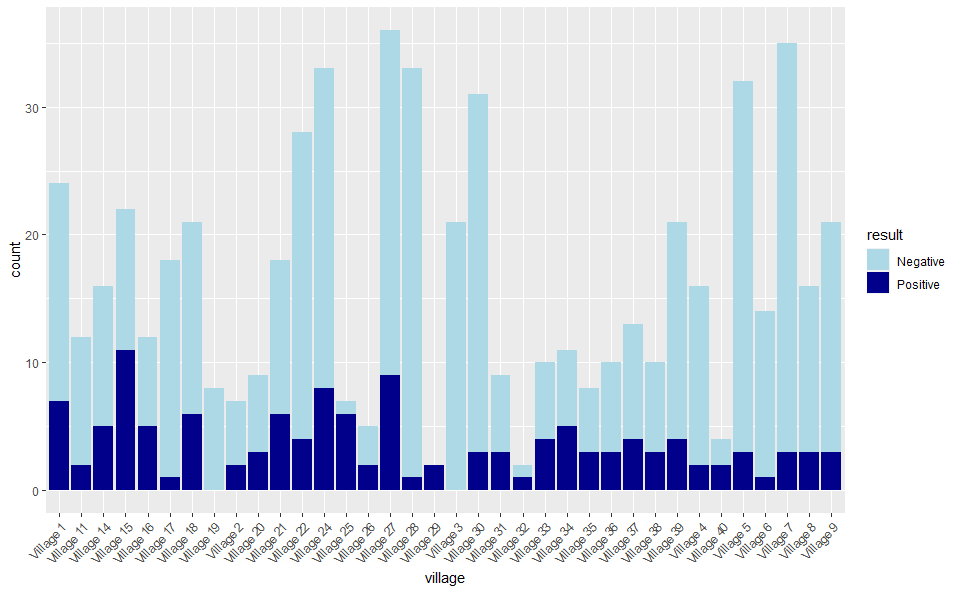
\includegraphics[width = 0.75\textwidth]{Images/village.png}
	\caption{Stacked bar plots of \texttt{result} in \texttt{village}}
	\label{fig:village} 
\end{figure}

\begin{table}[!h]
	\centering
	\begin{tabular}{|c|c|c|c|c|c|}
		\hline
		category & prevalence & category & prevalence & category & prevalence \\
		\hline
		Village 1 & 0.2917 & Village 16 & 0.4167 & Village 29 & 1.0000 \\
		Village 2 & 0.2857 & Village 17 & 0.0556 & Village 30 & 0.0968 \\
		Village 3 & 0 & Village 18 & 0.2857 & Village 31 & 0.3333 \\
		Village 4 & 0.1250 & Village 19 & 0 & Village 32 & 0.5000 \\
		Village 5 & 0.0938 & Village 20 & 0.3333 & Village 33 & 0.4000 \\
		Village 6 & 0.0714 & Village 21 & 0.3333 & Village 34 & 0.4545 \\
		Village 7 & 0.0857 & Village 22 & 0.1429 & Village 35 & 0.3750 \\
		Village 8 & 0.1875 & Village 24 & 0.2424 & Village 36 & 0.3000 \\		
		Village 9 & 0.1429 & Village 25 & 0.8571 & Village 37 & 0.3077 \\
		Village 11 & 0.1667 & Village 26 & 0.4000 & Village 38 & 0.3000 \\
		Village 14 & 0.3125 & Village 27 & 0.2500 &	Village 39 & 0.1905 \\
		Village 15 & 0.5000 & Village 2 & 0.0303 & Village 40 & 0.5000	\\
		\hline			
	\end{tabular}
	\caption{Prevalence in each category of \texttt{village}}
	\label{tab:village}
\end{table}

\begin{figure}[!h]
	\centering
	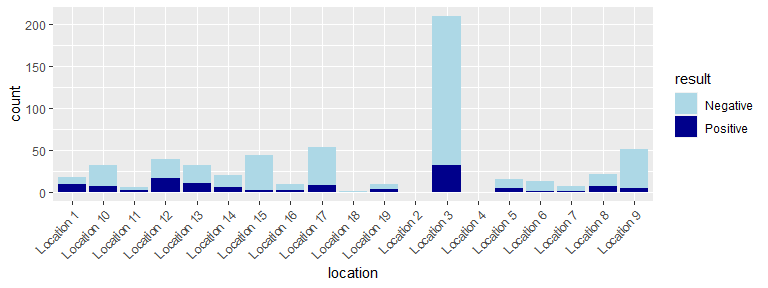
\includegraphics[width = 0.75\textwidth]{Images/location.png}
	\caption{Stacked bar plots of \texttt{result} in \texttt{location}}
	\label{fig:location}
\end{figure}

\begin{table}[!h]
	\centering
	\begin{tabular}{|c|c|c|c|c|c|}
		\hline
		category & prevalence & category & prevalence & category & prevalence \\
		\hline
		Location 1 & 0.5556 & Location 7 & 0.2857  & Location 13 & 0.3333 \\
		Location 2 & 1.0000	 & Location 8 & 0.3182 & Location 14 & 0.2857 \\
		Location 3 & 0.1571 & Location 9 & 0.0962 & Location 15 & 0.0667 \\
		Location 4 & 1.0000 & Location 10 & 0.2424 & Location 16 & 0.3000 \\
		Location 5 & 0.3125 & Location 11 & 0.5000 & Location 17 & 0.1667 \\
		Location 6 & 0.1429 & Location 12 & 0.4250 & Location 18 & 0.0000 \\
		 & & & & Location 19 & 0.4000 \\	
		\hline			
	\end{tabular}
	\caption{Prevalence in each category of \texttt{location}}
	\label{tab:location}
\end{table}

\begin{figure}[!h]
	\centering
	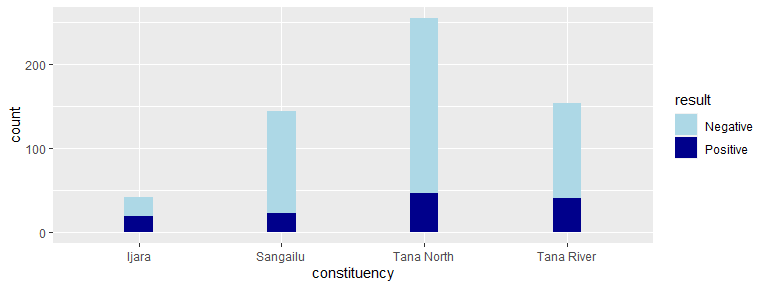
\includegraphics[width = 0.75\textwidth]{Images/constituency.png}
	\caption{Stacked bar plots of \texttt{result} in \texttt{constituency}}
	\label{fig:constituency}
\end{figure}	

\begin{table}[!h]
	\centering
	\begin{tabular}{|c|c|c|c|}
		\hline
		category & prevalence & category & prevalence \\
		\hline
		Tana North & 0.1843 & Tana River & 0.2662 \\
		Ijara & 0.4524 & Sangailu & 0.1597 \\
		\hline			
	\end{tabular}
	\caption{Prevalence in each category of \texttt{constituency}}
	\label{tab:constituency}
\end{table}

Nested structures are observed in environmental variables and we would like to take the influence of them into consideration due to great difference of prevalence among groups. However, we might consider the random effect of these variables rather than fixed effect, due to the hierarchical structures with numbers of levels in \texttt{village} and \texttt{location}. Models with random effect will be explained in the next section.

So far, we have extracted a subset for modelling with 595 observations, including 8 feature candidates and 3 environmental variables.

\clearpage

\section{Implementation}
\label{sec:implementation}

\subsection{Generalized Linear Mixed Model}

The exposition in this subsection follows that in Zuur (2009) \cite{zuur2009mixed}.

\

Since the response variable in our model is binomial, we start with the generalized linear model (GLM) for binomial data, i.e. logistic regression. 

Suppose the response $\boldsymbol{Y} = (Y_1, \cdots, Y_n)$ $Y_i \sim Bin(1, p_i)$, we have: 

$$logit(p_i) = ln \frac{p_i}{1-p_i} = \boldsymbol{x}_i^T\boldsymbol{\beta}$$

GLMs do not always work well. Sometimes data may contain multiple levels, which is known as nested or hierarchical structure, and data in each level may be correlated. In this case, regression results in different levels could vary and model assumptions such as homogeneity could be violated. To deal with it, we consider an extended model where part of parameters could change across different levels in the hierarchical variables (random effect), and the rest parameters keep consistent across levels (fixed effect). The GLM including both fixed and random effect is called the generalized linear mixed model (GLMM). 

Now, for the binomial GLMM for response $\boldsymbol{Y}$, we have:

$$logit(\boldsymbol{p})  = \boldsymbol{X}\boldsymbol{\beta} + \boldsymbol{Z}\boldsymbol{b} + \boldsymbol{\epsilon}$$

Here, $\boldsymbol{p} = (p_{ij})$ is matrix where $p_{ij}$ denotes the probability for individual $i$ in level $j$; $\boldsymbol{X}$ and $\boldsymbol{\beta}$ are the fixed effects design matrix and fixed effect respectively; $\boldsymbol{Z}$ and $\boldsymbol{b}$ are the random effects design matrix and random effect respectively; $\boldsymbol{\epsilon}$ is the matrix for unexplained information. Note that $\boldsymbol{b}$ and $\boldsymbol{\epsilon}$ follow normal distributions with mean 0. 

Besides the allowance for correlations among observations and nested data structure, GLMMs also reduce the model complexity. If we include the hierarchical variables with numerous levels in the fixed structure, we will obtain complicated models without stable results and generality. Considering the random effect instead only requires one extra parameter and can obtain more general statements. That's why we consider the random effect of environmental variables rather than their fixed effect.

\subsection{Model Construction and Selection}

\subsubsection{Step 1: Initial Model}

We start with a binomial GLM, containing feature candidates except geographical variables. Here, we do not contain the interaction terms of variables in the model as we do not detect much interaction among features. 

\subsubsection{Step 2: Find the Optimal Fixed Structure}

The \texttt{summary} and \texttt{step} function are both used to determine the optimal fixed structure among candidates. The latter function chooses the optimal model and significant features by AIC and the $\chi^2$ test. Table \ref{tab:summary1} and \ref{tab:step1} display the output of two functions.

\begin{table}[!h]
	\centering
	\begin{tabular}{|c|c|c|}
		\hline
		 & $t$ value & Pr($>|t|$) \\
		\hline
		\texttt{(Intercept)} & -0.341 & 0.73317 \\
		\texttt{genderMale} & -2.428 & \ \ \ 0.01520 * \\
		\texttt{age} & -1.798 & \ \ 0.07219 . \\
		\texttt{occupationHousewife} & -0.757 & 0.44890 \\  
		\texttt{occupationPastoralist} & 0.754 & 0.45068 \\   
		\texttt{occupationStudent} & -1.423 & 0.15463 \\  
		\texttt{landusepastoral} & -2.347 & \ \ \ 0.01892 * \\ 
		\texttt{landuseriverine} & -1.607 & 0.10810 \\   
		\texttt{altitude} & -1.681 & \ \ 0.09283 . \\
		\texttt{famsize} & 0.346 & 0.72900 \\   
		\texttt{hhoccupPastoralist} & 3.181 & \ \ \ \ 0.00147 ** \\
		\texttt{disthosp} & 0.301 & 0.76322 \\   
		\hline
		\multicolumn{3}{|l|}{Significance codes: 0,\ ‘***’ 0.001,\ ‘**’ 0.01,\ ‘*’ 0.05,\ ‘.’ 0.1,\ ‘ ’ 1} \\
		\hline
	\end{tabular}
	\caption{Feature significance in initial GLM using \texttt{summary} function}
	\label{tab:summary1}
\end{table}

\begin{table}[!h]
	\centering
	\begin{tabular}{|c|c|c|c|}
		\hline
		 & Df & AIC & Pr($>$Chi) \\
		\hline
		\texttt{(none)} & & 602.72 & \\                      
		\texttt{altitude} & 1 & 603.45 & 0.0990659 . \\ 
		\texttt{age} & 1 & 603.86 & 0.0765869 . \\ 
		\texttt{landuse} & 2 & 604.59 & 0.0531339 . \\ 
		\texttt{occupation} & 3 & 605.55 & \ 0.0316715 * \\ 
		\texttt{gender} & 1 & 606.75 & \ 0.0141019 * \\ 
		\texttt{hhoccup} & 1 & 611.90 & \ \ \ \ 0.0008302 *** \\
		\hline
		\multicolumn{4}{|l|}{Significance codes: 0,\ ‘***’ 0.001,\ ‘**’ 0.01,\ ‘*’ 0.05,\ ‘.’ 0.1,\ ‘ ’ 1} \\
		\hline
	\end{tabular}
	\caption{Significant features in stepwise algorithm using \texttt{step} function}
	\label{tab:step1}
\end{table}

We select \texttt{gender} and \texttt{hhoccup}, which are statistically significant at 0.05 significance level in the output of both functions. Besides, \texttt{landuse} is also selected, as it is significant at 0.1 significance level in stepwise selection and one of its levels is statistically significant at 0.05 level in model summary.  

Although \texttt{occupation} shows its significance in stepwise algorithm, none of its levels is significant in model summary. On the other hand, we observe high correlation between \texttt{occupation} and \texttt{landuse}, which probably causes collinearity and poor model performance. Therefore, we do not include \texttt{occupation} in the fixed structure.

In conclusion, the optimal fixed structure consists of \texttt{gender}, \texttt{landuse} and \texttt{hhoccup}.

\subsubsection{Step 3: Find the Optimal Random Structure}

With the optimal fixed structure, we now introduce the random effect of environmental variables and determine GLMM with the best performance, using R package \texttt{lme4} \cite{lme4}. As mentioned, we investigate whether there is a village or location effect. 

We start with fitting the random intercept model of \texttt{village}. To assess whether the model with mixed effect model is better than the ordinary binomial GLM, we refit the latter one over the selected features without random intercept and compare the models using \texttt{anova} function. The output is given in Table \ref{tab:glmm1}:

\begin{table}[!h]
	\centering
	\begin{tabular}{|c|c|c|c|c|c|c|c|c|}
		\hline
		 & npar & AIC & BIC & logLik & deviance & Chisq & Df & Pr($>$Chisq) \\  
		 \hline
		GLM & 5 & 603.63 & 625.57 & -296.81 & 593.63 & & & \\                      
		GLMM(\texttt{village}) & 6 & 601.87 & 628.20 & -294.93 & 589.87 & 3.7611 & 1 & 0.05246 . \\
		\hline
		\multicolumn{9}{|l|}{Significance codes: 0,\ ‘***’ 0.001,\ ‘**’ 0.01,\ ‘*’ 0.05,\ ‘.’ 0.1,\ ‘ ’ 1} \\
		\hline
	\end{tabular}
	\caption{Comparison between GLM and GLMM of \texttt{village}}
	\label{tab:glmm1}
\end{table}

Lower AIC value indicates that the mixed model including village effect is preferred. Moreover, we extend the random part by adding random slopes. Specifically, the \texttt{landuse} effect may be different per village and the same may hold for the \texttt{hhoccup} effect. Table \ref{tab:glmm2} show the output of model comparison using \texttt{anova} function:

\begin{table}[!h]
	\centering
	\begin{tabular}{|c|c|c|c|c|c|c|c|c|}
		\hline
		& npar & AIC & BIC & logLik & deviance & Chisq & Df & Pr($>$Chisq) \\  
		\hline
		random intercept & 6 & 601.87 & 628.20 & -294.93 & 589.87 & & & \\                      
		random intercept + \texttt{landuse} & 8 & 605.75 & 640.85 & -294.87 & 589.75 & 0.122 & 2 & 0.9408 \\
		random intercept + \texttt{hhoccup} & 11 & 611.48 & 659.76 & -294.74 & 589.48 & 0.264 & 3 & 0.9667 \\
		\hline
		\multicolumn{9}{|l|}{Significance codes: 0,\ ‘***’ 0.001,\ ‘**’ 0.01,\ ‘*’ 0.05,\ ‘.’ 0.1,\ ‘ ’ 1} \\
		\hline
	\end{tabular}
	\caption{Comparison among GLMMs of \texttt{village} with different random structures}
	\label{tab:glmm2}
\end{table}

Extending the model with random slopes gives no improvement as the AIC values of models with random slopes get higher. Now we consider the alternative model with the random intercept of \texttt{location}. Comparison between random intercept models of \texttt{village} and \texttt{location} by AIC is displayed in Table \ref{tab:glmm3}:

\begin{table}[!h]
	\centering
	\begin{tabular}{|c|c|c|}
		\hline
		& df & AIC  \\  
		\hline
		GLMM(\texttt{village}) & 6 & 601.8683	\\	
		GLMM(\texttt{location}) & 6 & 601.8942 \\
		\hline
	\end{tabular}
	\caption{Comparison between random intercept models of \texttt{village} and \texttt{location}}
	\label{tab:glmm3}
\end{table}

The AIC value of the random intercept model with the village effect is slightly lower. Besides, since the column \texttt{village} contains more levels than \texttt{location}, the models considering the random effect on village aspect obtain more detailed results. The random intercept and slope models of \texttt{location} performs even worse. Consequently, we choose the random intercept model with village effect as the optimal model.

\

Note that we do not consider the constituency effect as \texttt{constituency} only contains 4 levels. It might be better to include this variable in model's fixed structure. However, after introducing the fixed effect of \texttt{constituency}, other variables in the fixed structure become insignificant. Moreover, the standard deviation of the random village or location effect turns to 0, indicating no difference among villages or locations. Thus, the influence of \texttt{constituency} is ruled out.

\clearpage

\section{Results}
\label{sec:results}

\subsection{Model Diagnosis} 

In linear regressions, we usually look at the residual plots and normal Q-Q plots to check if the model assumptions are satisfied. However, these are probably not suitable for GL(M)Ms. Standard residual plots, when interpreted in the same way as for linear models, seem to show all kind of problems, such as non-normality, heteroscedasticity, even if the model is correctly specified. For example, the standard residual plot of our optimal model, shown in Figure \ref{fig:std_resplot}, has an obvious pattern. In this case, we get confused and are not able to tell whether such pattern in GLMM residuals is a problem or not.

\begin{figure}[!h]
	\centering
	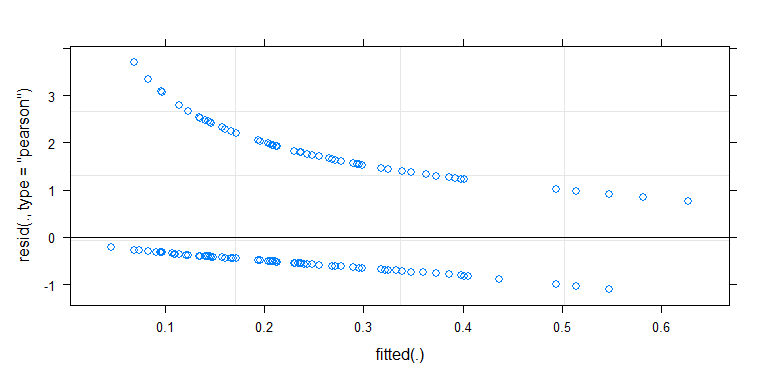
\includegraphics[width = 0.75\textwidth]{Images/std_resplot.png}
	\caption{Standard residual plot of the optimal model}
	\label{fig:std_resplot}
\end{figure}

To address this problem, we adopt the \texttt{DHARMa} package \cite{dharma}. It aims to create readily interpretable residuals for GL(M)Ms that are standardized to values between 0 and 1. \texttt{DHARMa} also provides Q-Q plots to detect overall deviations from the expected distribution. The basic steps are:

\begin{enumerate}
	\item Simulate new response data from the fitted model.
	\item Calculate the empirical cumulative density function for the simulated observations, which describes the possible values (and their probability) at the predictor combination of the observed value, assuming the fitted model is correct.
	\item The residual is then defined as the value of the empirical density function at the value of the observed data.
\end{enumerate}

We simulate 1000 observations based on our optimal model, and plot the scaled residuals. Intuitively, nothing in the Figure \ref{fig:diagnosis1} is highlighted in red, indicating no violation of model assumptions is detected. Specifically, well-performed Q-Q plot indicates that the residuals are normally distributed. In the residual plot on the right, we do not observe obvious pattern of scaled residuals. As a result, we do not detect significant problems in the optimal model.

\begin{figure}[!h]
	\centering
	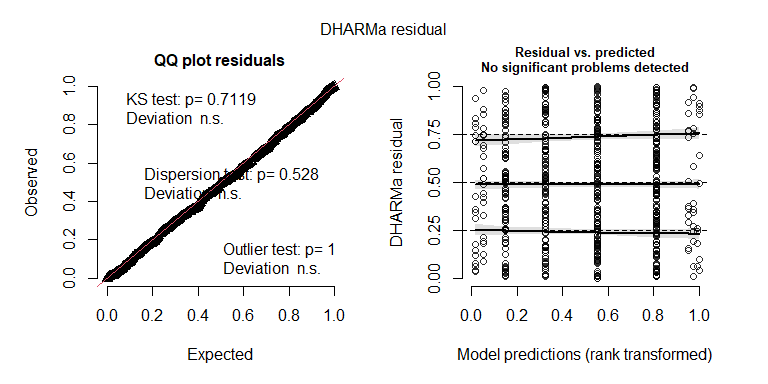
\includegraphics[width = 0.75\textwidth]{Images/diagnosis1.png}
	\caption{\texttt{DHARMa} residual plot and Q-Q plot of the optimal model}
	\label{fig:diagnosis1}
\end{figure}

Besides, as recommended in \cite{dharma}, we plot the residuals against specific predictors including \texttt{landuse} and \texttt{occuparion} in Figure \ref{fig:diagnosis2}. Again, no significant problem is detected.

\begin{figure}[!h]
	\centering
	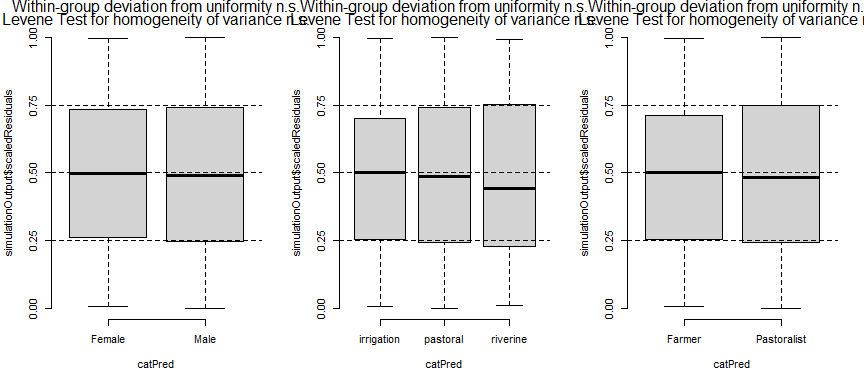
\includegraphics[width = 0.75\textwidth]{Images/diagnosis2.png}
	\caption{\texttt{DHARMa} residual plot and Q-Q plot of the optimal model}
	\label{fig:diagnosis2}
\end{figure}

\subsection{Model Evaluation}

Due to binomial response, for model evaluation, we plot the ROC (Receiver Operating Characteristic) curve and compute the corresponding AUC (Area Under Curve) value with 95\% confidence intervals using R package \cite{proc}. We repeat the same steps for the ordinary GLM and the random intercept model with location effect. Furthermore, we compute the mean AUC of models using 10-fold cross validation using R package \texttt{caret} \cite{caret}. 

\begin{figure}[!h]
	\centering
	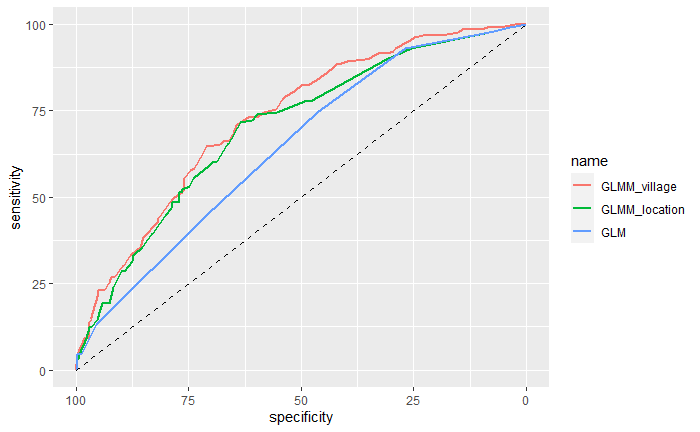
\includegraphics[width = 0.75\textwidth]{Images/ROC.png}
	\caption{ROC curves of models} 
	\label{fig:pROC}
\end{figure}

\begin{table}[!h]
	\centering
	\begin{tabular}{|c|c|c|c|}
		\hline
		 & AUC & 95\% CI & meanAUC in 10-fold CV\\
		\hline
		GLMM(\texttt{village}) & 0.7275 & (0.6806, 0.7745) & 0.6687 \\
		GLMM(\texttt{location}) & 0.7018 & (0.6520, 0.7516) & 0.6681 \\
		GLM & 0.6437 & (0.5942, 0.6932) & 0.6454 \\
		\hline	
	\end{tabular}
	\caption{AUC values of models}
	\label{tab:AUC}
\end{table}

According to Figure \ref{fig:pROC} and Table \ref{tab:AUC}, ROC curve beyond the random baseline and $AUC = 0.7275 > 0.5$ indicate good performance of the optimal model. Moreover, the random intercept model with village effect over-performs the rest two models, implying its better ability to explain and predict. 

\subsection{Model Interpretation}

Table \ref{tab:summary2} and Table \ref{tab:summary3} display the detailed model summary.

\begin{table}[!h]
	\centering
	\begin{tabular}{|c|c|c|c|c|}
		\hline
		 & Estimate & Std.Error & $t$ value & Pr($>|t|$) \\
		\hline
		\texttt{(Intercept)} & -1.6179 & 0.2589 & -6.249 & \ \ \ \ \ 4.13e-10 *** \\
		\texttt{genderMale} & -0.4421 & 0.2141 & -2.065 & \ \ 0.03895 * \\  
		\texttt{landusepastoral} & -1.0268 & 0.5697 & -1.802 & \ \ 0.07148 . \\ 
		\texttt{landuseriverine} & -0.5554 & 0.5850 & -0.949 & 0.34245 \\    
		\texttt{hhoccupPastoralist} & 1.8716 & 0.5401 & 3.465 & \ \ \ \ \ 0.00053 *** \\
		\hline
		\multicolumn{5}{|l|}{Significance codes: 0,\ ‘***’ 0.001,\ ‘**’ 0.01,\ ‘*’ 0.05,\ ‘.’ 0.1,\ ‘ ’ 1} \\
	    \hline
	\end{tabular}
	\caption{Summary of the fixed effect}
	\label{tab:summary2}
\end{table}

\begin{table}[!h]
	\centering
	\begin{tabular}{|c|c|c|c|}
		\hline
		Groups & Name & Variance & Std.Dev. \\
		\hline
		\texttt{village} & (Intercept) & 0.2553 & 0.5053 \\
		\hline
	\end{tabular}
	\caption{Summary of random effect}
	\label{tab:summary3}
\end{table}

\texttt{gender}, \texttt{hhoccup} and \texttt{landuse} (0.1 significance level) show significant influence on leptospirosis seropositivity, hence they are considered as risk factors for leptospirosis. The optimal model is given by:
\begin{align*}
	Y_{ij} & \sim Bin(1, p_{ij}) \\
	logit(p_{ij}) &=  -1.6179 - 0.4421 \times \mathbb{I}(\texttt{gender}_{ij} = Male)  \\
	& \ \ \ \ - 1.0268 \times \mathbb{I}(\texttt{landuse}_{ij} = pastoral) - 0.5554 \times \mathbb{I}(\texttt{landuse}_{ij} = riverine) \\
	& \ \ \ \ + 1.8176 \times \mathbb{I}(\texttt{hhoccup}_{ij} = Pastoralist) + v_i \\
	v_i & \sim N(0, 0.5053^2)
\end{align*}	

Here, $Y_{ij}$ denotes the test result of individual $j$ in village $i$, with the probability $p_{ij}$. The notation \emph{logit} stands for the logistic link function. The notation $\mathbb{I}$ represents the indicator function, with the general expression:

\begin{equation*}
	\mathbb{I}_X(x) = 
	\begin{cases}
		1, \quad if \ x \in X \\
		0, \quad if \ x \notin X	
	\end{cases}
\end{equation*}

$v_i$ denotes the random intercept across villages, following a Normal distribution with mean $\mu = 0$ and standard deviation $\sigma = 0.5053$, indicating that the majority of the values (95\% to be more exact) of $v_i$ fall between $(-1.96 \times 0.5053, 1.96 \times 0.5053)$.  

For example, a male individual from Village 1, with riverine land and household head occupation "Farmer", has a probability $p$ of being leptospirosis seropositive, where $p$ satisfies:

$$ logit(p) = ln \frac{p}{1-p} =  -1.6179 - 0.4421 - 0.5554 + v_1 = -2.6154 + v_1, \quad v_1 \sim N(0, 0.5053^2)$$

Based on \cite{jewell2003statistics} and \cite{zuur2009mixed}, the intercept terms including $v_i$ denote the log odds of leptospirosis seropositivity in the baseline model. The reference groups for features in the fixed structure are $\texttt{gender} = Female$, $\texttt{landuse} = irrigation$, and $\texttt{hhoccup} = Farmer$. In village $i$, we have 

$$odds_{\texttt{result}} = \frac{P(Positive \ | \ female, irrigation, farmer)}{P(Negative \ | \ female,  irrigation, farmer)} \
										= e^{-1.6179 + v_i} 
										\approx 0.1983 \times e^{v_i} $$
										
Particularly, considering an average village effect, i.e. $v_i = 0$, we obtain an average odds 0.1983 for leptospirosis seropositivity in the baseline model above, with the 95\% confidence interval $(0.1159, 0.3316)$. 

~\\
Holding the average village effect, we have the odds ratios of factors with 95\% confidence intervals:

\begin{itemize}
	\item With \texttt{landuse} and \texttt{hhoccup} fixed, the odds of leptospirosis seropositivity for those in male group is 0.6427 (0.4194, 0.9764) times the odds of those in female group. Male individuals take less risk for leptospirosis seropositivity, probably because they have better resistance and immunity than females.
	
	\item With \texttt{gender} and \texttt{hhoccup} fixed, the odds of leptospirosis seropositivity for those working on pastoral land is 0.3582 (0.1151, 1.1372) times the odds of those working on irrigation land; the odds of leptospirosis seropositivity for those working on riverine land is 0.5738 (0.1657, 1.8141) times the odds of those working on irrigation land. People working on the irrigation land contact more with both polluted water and animal urine, which may contain the bacteria, and have higher risk for leptospirosis infection \cite{farr1995leptospirosis}. 
	
	\item With \texttt{gender} and \texttt{landuse} fixed, the odds of leptospirosis seropositivity for people whose household heads work as pastoralists is 6.4987 (2.2190, 19.3265) times the odds of those in farmers group. Comparing with farmers, pastoralists have more contact with animals and are more likely to be exposed to the bacteria. Further, leptospirosis has higher probability to be spread in the households of pastoralists. 
	
\end{itemize}

\clearpage

\section{Conclusions}

We extract a subset of the data sampled from households in villages of Tana River County, Kenya, and construct a generalized linear mixed model including the random effect of villages, to identify risk factors on leptospirosis. As a result, individual's gender, land use type (0.1 significance level) and the occupation of household head appear to have significant influence on the seropositivity of leptospirosis. Specifically, male individuals seem to have lower risk of transmission of this zoonotic disease. People from household with the irrigation land are most likely to be infected, comparing with those from household with pastoral or riverine land. Besides, members from a household with the head working as a pastoralist tends to take more risk for leptospirosis seropositivity than those from a household with the head working as a farmer.

There are several limitations of this research. First, we delete over 300 observations in EDA section, due to missing or other problems, which leads to a great loss of information and further possibly biased model results. We expect improvement of model accuracy and performance, based on more complete dataset with less mistakes. Second, the response column for ELIZA test result has an imbalanced distribution where most observations have negative results. This may result in model bias as our classifier tends to over-adapt to the negative group. In this case, a possible future research could be the exploration of zero-inflated models on the count data, by concerting the observations from individual to household aspects. Moreover, we could explore the models using Bayesian methods with proper and informative priors in future.

\clearpage

%the entries have to be in the file literature.bib
\bibliographystyle{unsrt}
\bibliography{literature}
\clearpage

\appendix
\section*{Appendix}
\addcontentsline{toc}{section}{Appendix}

Programming part in this research is completed with R. 

\subsection*{R packages:}

For EDA section, we use the \texttt{tidyverse} and \texttt{gridExtra} packages. We construct models with \texttt{lme4} package. \texttt{DHARMa} package is used for model diagnosis. \texttt{pROC} and \texttt{caret} packages are used for model evaluation. All histograms and line graphs are generated with \texttt{ggplot2}.

\subsection*{R code: }
The complete code is available via this \href{https://github.com/Shi-Yile/Project-2-Leptospirosis-Risk-Factors.git}{Github repository}.

\clearpage

\section*{Word Count}
\addcontentsline{toc}{section}{Word Count}

This report contains 4987 words, including executive summary, main text, and references. The screenshot using \texttt{Analyse Text} function in TeXstudio is provided.

\begin{figure}[!h]
	\centering
	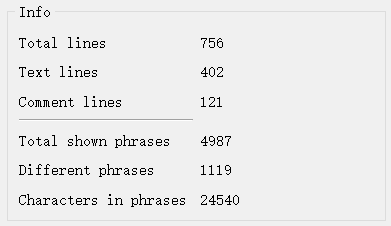
\includegraphics[width = 0.75\textwidth]{Images/wordcount.png}
	\caption{Word count in TeXstudio}
	\label{fig:wordcount}
\end{figure}

\end{document}
